\documentclass[10pt]{article}

\usepackage{verbatim}
\usepackage{times}
\usepackage{amsmath}
\usepackage{amsthm}
\usepackage{amssymb}
\usepackage{multirow}
\usepackage{graphicx}
\usepackage{dcolumn}
\usepackage{cite}
\usepackage{epstopdf}
\usepackage{hyperref}






\title{A Visual Proof Of The Pythagorean Theorem}
%Mine proof of pythagoras
\author{Pythagoras}
%name of mine
\date{\today}
%todays date
%
\makeatletter
    \setlength\@fptop{0\p@}
\makeatother
\begin{document}
\maketitle
\section{\underline{Introduction}}
\label{sec:intro}
The theorem is of fundamental importance in Euclidean Geometry where it serves as a basis for the definition of distance between two points.\emph{The area of the square built upon the hypotenuse of a right triangle is equal to the sum of the areas of the squares upon the remaining sides}.
\section{\underline{Theorem, Definition And Relation}}
\label{sec:def}
\newtheorem{mydef}{Theorem}[section]
\begin{mydef}
The square of the hypotenuse (the side opposite the right angle) is equal to the sum of the squares of the other two sides (base and height).
\end{mydef}
\newtheorem{mydef2}{Definition}[section]
\begin{mydef2}
The theorem that the sum of the squares of the lengths of the sides of a right triangle is equal to the square of the length of the hypotenuse.
\end{mydef2}
In mathematics, the Pythagoras theorem or Pythagorean theorem is a relation in Euclidean geometry among the three sides of a right triangle. The theorem can be written as an equation relating the lengths of the sides a, b and c of a right angled triangle, often called the Pythagorean equation:
\begin{equation}
\label{one}
a^2+b^2=c^2
\end{equation}
where c represents the length of the hypotenuse, and a and b represent the lengths of the other two sides.


\section{\underline{Importance of Pythagoras theorem}}
\label{sec:importance}

There are many uses for the Pythagorean Theorem, that is the main reason and is important. You can use the Pythagorean Theorem to find out if a triangle is an acute triangle, obtuse triangle or a right triangle. If the Theorem works and the side lengths squared is equal to the hypotenuse squared, then it is a right triangle, if the hypotenuse squared is longer than the two side lengths squared and added together then the triangle is obtuse. If the hypotenuse squared is shorter than the two side lengths squared and added together then the triangle is acute.\newline
Another reason the Pythagorean Theorem is imported is it can help you find missing side lengths. Not only can it help you find the third side length to a right triangle, but it can also help you find the missing side lengths to squares and rectangles when the triangles are pushed together. The pythagorean Theorem can help build rectangles and squares.

\section{\underline{Proof of the Pythagorean Theorem using Algebra}}
\label{sec:proof}

We can show that using Algebra....\newline
Take a look at the diagram shown below ... it has that "abc" triangle in it (four of them actually)........

\begin{figure}[htb!]
  \begin{center}
    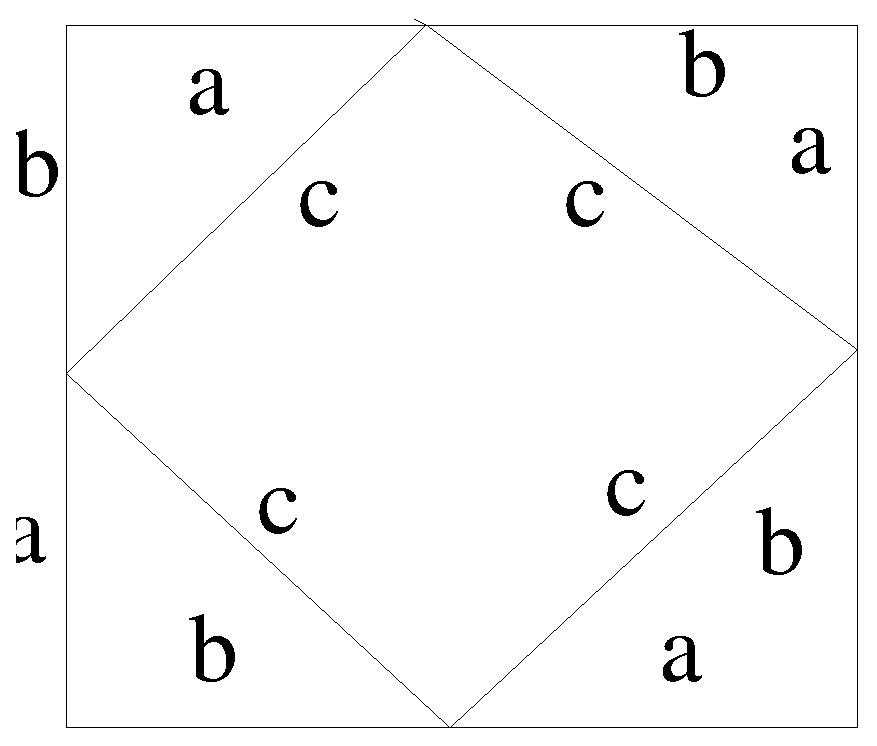
\includegraphics[width=0.5\columnwidth]{fig9.eps}
   \end{center}
  \caption{Figure for pythagoras theorem}
  \label{image1}
\end{figure}
Figure~\ref{image1} shows a photo of a square contains various figures. We will calculate the areas of the respective figures in the below subsections.


\subsection{\underline{Area of Whole Square}}
\label{a_square}

It is a big square, with each side having a length of a+b, so the total area is:

$$A = (a+b)(a+b)$$

\subsection{\underline{Area of Other Pieces}}
\label{a_pieces}

Now let's add up the areas of all the smaller pieces:\newline
First, the smaller (tilted) square has an area of:
\begin{equation}
\label{two}
A = c^2 
\end{equation} 
And there are four triangles, each one has an area of 
\begin{equation}
\label{three}
A =\frac{1}{2} ab
\end{equation}
So all four of them combined is	
\begin{equation}
\label{two}
A = 4(\frac{1}{2}ab) = 2ab
\end{equation} 
So, adding up the tilted square and the 4 triangles gives: 
\begin{equation}
\label{five}
A = c^2 +2ab
\end{equation}


\subsection{\underline{Both Areas Must Be Equal}}
\label{a_equal}

The area of the large square is equal to the area of the tilted square and the 4 triangles. This can be written as (from equation ~\ref{five}):\newline
\begin{equation}
\label{six}
(a+b)(a+b) = c^2 +2ab
\end{equation}
Now, let us rearrange equation ~\ref{six} to see if we can get the pythagoras theorem:
\begin{equation}
\label{seven}
(a+b)(a+b)	=	c^2 + 2ab
\end{equation}
Expand (a+b)(a+b) in equation ~\ref{seven}:
\begin{equation}
\label{eight}
a² + 2ab + b²	=	c^2 + 2ab
\end{equation}
Subtract "2ab" from both sides in equation ~\ref{eight}:\newline	 
\centerline {$a^2$ + $b^2$	=	$c^2$}\newline

The following above statements gives us the proof of 
pythagoras theorem. Also, we can see the table below to see the correctness of theorem.

\section{\underline{Examples in Tabular Form}}
\begin{table}[bht]%\Large
	\begin{center}
		\begin{tabular}{c c c c c c c}
			\hline\hline
			Lenght a & Height b & Hypotenuse c & $a^2$ & $b^2$ & $c^2$ & $a^2$+$b^2$    \\
			\hline
			\hline
			4 & 3 & 5 & 16 & 9 & 25 & 25 \\
			8 & 15 & 17 & 64 & 225 & 289 & 289\\
			9 & 40 & 41 & 81 & 1600 & 1681 & 1681\\
			5 & 12 & 13 & 25 & 144 & 169 & 169 \\
			7 & 24 & 25 & 49 & 576 & 625 & 625\\
			\hline
		\end{tabular}
		%hsgdflg
		\caption{Examples}
		\label{sec:examp}
	\end{center}
\end{table}
\clearpage
\nocite{*}
\bibliographystyle{plain}
\bibliography{a1}











\end{document}
